\documentclass[]{assignment}

\begin{document}


%%% INPUT YOUR NAME AND STUDENT NUMBER
%%% INPUT YOUR NAME AND STUDENT NUMBER
%%% -->
\def\studentname{James Dorrian}
\def\ucdstudentnumber{13369451}
%%% <--

%%%%%%%%%%%%%%%%%%%%%%
%%% 1st Section

\section{{\bf First Assignment:} Image Processing and Coding}

%%% First Sub-Section
\subsection{Image Filters} 

Part one of this section involves filtering the image by means of histogram modification. The pixels $(R,G,B)$ are processed individually to perform contrast enhancement. The transformation is independent of the colour channel and pixel location.

There are the 3 histogram transformation functions, and $(R_F,G_F,B_F)$.

First we normalise the pixel values in the range $[0\ldots 1]$.
Then multiply each histogram transformation function by the briselames image. We use the $polyval()$ function which gives us the polynomial coefficients of the histogram function. We then multiply by 255 to move back to the correct color spectrum $[0\ldots 255]$

Now we have 3 distinct color channels and we can combine them to create our new image. Note, we must first convert each layer to uint8 as doubles cannot be displayed. To achieve out desired image $fig.1(c)$ we must concatenate the 3 layers.


\begin{figure}[h]
\centering
\fboxsep 0mm
\parbox{5cm}{\framebox{\includegraphics[width=5cm]{I_original}}\\\centering{(a)}}
~~~
\parbox{5cm}{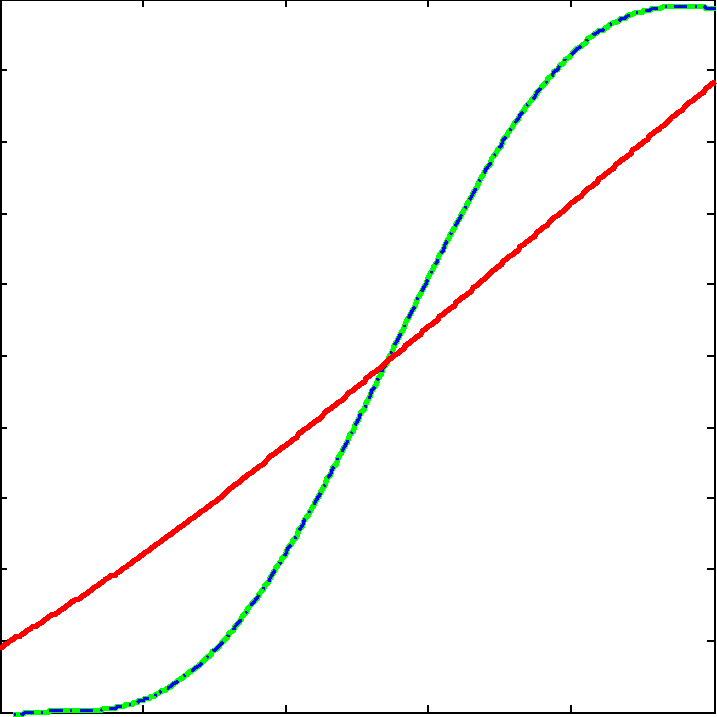
\includegraphics[width=5.05cm]{Trgb.pdf}\\\centering{(b)}}
~~~
\parbox{5cm}{\framebox{\includegraphics[width=5cm]{I_hist_proc}}\\\centering{(c)}}
\caption{\label{fig:imgfilter1} Original image (a), histogram transformation function (b), and filtered image (c).}
\end{figure} 

The second part of the filter involves combining the filtered image seen in $(c)$ above with a radial gradient image. To do this we got the centre of the image (width/2, height/2) and checked how far away every pixel in the image was from this point (distance formula). We used the distance to apply the formula found below to each pixel location and then saved those values in an array of the same size as our original image. The formula states that pixels are assigned the value 0.5 if under 1/3 from center (gray) and assigned the value 0 (black) if over 2/3 from center. A function defines a smooth blend from gray to black for all pixels between 1/3 and 2/3 away from the center.


$C(\rho) = 
\left\{ \begin{array}{lcl}
1/2  & ~~~\mbox{for}~ &\rho < 1/3\\
\displaystyle \frac{1+\cos 3 \pi (\rho-1/3)}{4}  & ~~~\mbox{for}~ &\rho\in [1/3\ldots 2/3]\\
0  & ~~~\mbox{for}~ &\rho> 2/3
\end{array}
\right.$


Where $\rho$ is the normalised distance from the centre

\clearpage

\begin{figure}[h]
\centering
\fboxsep 0mm
\parbox{5cm}{\framebox{\includegraphics[width=5cm]{blend_img}}\\\centering{(a)}}
~~~
\parbox{5cm}{\framebox{\includegraphics[width=5cm]{I_hist_proc_blend}}\\\centering{(b)}}
\caption{\label{fig:imgfilter2} Vignette Image (a) and combined image (vignette + filtered image) (b).}
\end{figure} 

$fig.2(a)$ seen above is the vignette gradient that we created using the distance from center algorithm above. Next we combine the briselames image seen in $fig.1(a)$ with the vignette. This is done using the non commutative blending mode and once again we treat each colour channel independently. This gives us a blended image. 

Next we pass this new image (called $combinedImage$ in my code) back into the histogram transformation function defined above. This transforms the histogram of our combined image and gives us our final result which is seen in $fig.2(b)$.  

%%% Second Sub-Section

\subsection{Block Transform} 

DCT (discrete cosine transformation) is a technique used in image compression which involves converting a signal into elementary frequency components. For the purposes of this assignment I used lena.png as the image on which I applied the DCT. 

The question wanted us to compute the DCT coefficients of 8x8 blocks of the original image and an image with 128 subtracted from all pixels. It wanted us to compare the range of the resulting values.



The first thing I did was create a dct transform matrix using a function known as $dctmtx$ and a block processing operation known as $blockProc$ to split the image up into 8$\times$8 pixel blocks. 

Next, I had to find the range of each block of both images and add the range of each block together in order to compare the original image with the modified image. 

The range of DCT values in the original image was: $4.2481e+06$
and the range of DCT values in the modified image was: $ 1.4304e+06 $

This is a difference in range of approximately $33.6715\%$. The reasoning behind the difference in range is that instead of the pixel range being from $[0\ldots 255]$ they are from $[128\ldots 127]$ .

By having 0 as the midpoint Quantisation and DCT operations are much more efficient.

\clearpage
%%% Third Sub-Section

\subsection{Quantization} 

My Quantisation method relies on the work we did using the DCT and splitting the image up into 8x8 blocks. We are trying to achieve lossy compression through the quantisation of DCT coefficients using an 'optimised quantization table' for the luminance components. This helps us minimize the Human perception of image degradation. 



My Quantization function has 2 input parameters:
\bin
\bb The block (8x8 block)
\bb The quality degradation parameter
\ein

The quality degradation parameter has a direct effect on our alpha value. Where the degradation parameter $\alpha = 1, 200-2\gamma, 5000/\gamma$  where $\gamma = 100, 50 \leq \gamma \leq 99, \gamma < 50$ respectively. 

The final quantized DCT coefficient matrix $\bf C$ is given by:

$C(i,j)=\mathrm{round}\left(\displaystyle\frac{B(i,j)}{\tilde{Q}(i,j)}\right)$ 

The histograms below are 2 sample blocks that have been quantized :

\begin{figure}[h]
\centering
\fboxsep 0mm
\parbox{6cm}{\framebox{\includegraphics[width=6cm]{block1}}\\\centering{(a)}}
~~~
\parbox{6cm}{\framebox{\includegraphics[width=6cm]{block125}}\\\centering{(b)}}
\caption{\label{fig:imgfilter1} Block number 1 (a) and Block number 125 (b)}
\end{figure} 


In $fig.3(a)$ we see a larger range than that seen in  $fig.3(b)$. 

Their ranges are $0 < X < 100$ and $-10 < X < 80$ respectively. 
\clearpage

%%% Fourth Sub-Section

\subsection{Zigzag Reordering} 

The zig-zag reordering algorithm that I used was found on stack overflow here: $(http://stackoverflow.com/questions/3024939/matrix-zigzag-reordering)$ 

This link was posted to the computer science 2013-2017 page as a reference for this question and I found it of great use in completing this section of the assignment. I found this post a great aid in the assignment and appreciate how very clear and concisely it is explained.

In essence what I learned from this post was that there is a super simple way to reorder a block into zigzag format and I have outlined it below:

\begin{enumerate}
  \item Get the linear index of each value in the array (column by column not row by row)
  \item Reverse the column order fliplr
  \item Use spdiags() to invert the array on the diagonal
  \item Reverse column order fliplr
  \item Use flipud() to reverse the order of the odd columns
  \item Keep only non-zero indices i.e. all those not added by spdiags()
  \item return Z as the reordered 8x8 block
\end{enumerate}

\begin{figure}[h]
\centering
\fboxsep 0mm
\framebox{\includegraphics[width=6cm]{zigzagscan}}
\caption{\label{fig:zigzag} The new zig-zag path}
\end{figure} 

\clearpage

\subsection{DPCM on DC component} 

First of all I got all the DC components from the 8x8 blocks and plotted them in a histogram. The DC component is the first component in the 8x8 block, and so it can be easily found and store using a simple counter and accessing the element in row 1 column 1. Displayed below is the histogram of my results:

Secondly I got the DC component of from the previous 8x8 block and subtracted it from the current 8x8 block and plotted that value. Displayed is the histogram of my results:

\begin{figure}[h]
\centering
\fboxsep 0mm
\parbox{7cm}{\framebox{\includegraphics[width=7cm]{hist1}}\\\centering{(a)}}
~~~
\parbox{7cm}{\framebox{\includegraphics[width=7cm]{hist2}}\\\centering{(b)}}
\caption{\label{fig:imgfilter1} The range of all DCT Values (a) and The difference of neighbouring DCT values (b)}
\end{figure} 

It is clear to see that there is much less differentiation between neighbours than that of non-neighbours. We can see that one of the most striking differences between these two histograms is the range of values. In $fig.5(b)$ most of the emphasis is around 0 meaning that there is very little variation between neighbours. When compared to the variation seen on the overall values $fig.5(a)$ this is very informative as it tells us that regions close together have similar pixel values. 

This is the whole point of compression and makes perfect sense as it is rational that pixels in the same region blend gradually into other colors. 


\label{last_page}

 \end{document} 